\documentclass[a4paper,DIV=12,english]{scrartcl}
\usepackage[utf8]{inputenc}
\usepackage{fancyhdr}
\usepackage{bookmark}
\usepackage{graphicx}
\usepackage{hyperref}
\usepackage{xurl}
\usepackage[sorting=none, style=numeric-comp]{biblatex}
\addbibresource{ref.bib}
\usepackage{csquotes}
\usepackage[dvipsnames]{xcolor}
\usepackage[num]{isodate}
\usepackage{amsthm}
\usepackage{amssymb}
\usepackage{bbm}
\usepackage{amsmath}
\usepackage{tikz}
%\usepackage{pgfplots}
    %\usepgfplotslibrary{fillbetween}
\usepackage{svg}
\usepackage{braket}
\usepackage{caption}
\usepackage{subcaption}
\usepackage{placeins}
%\setlength\parindent{0pt}
\usepackage{wrapfig}
\usepackage{float}


% Fakesection
\newcommand{\fakesection}[1]{%
    \par\refstepcounter{section}                                        % Increase section counter
    \sectionmark{#1}                                                    % Add section mark (header)
    \addcontentsline{toc}{section}{\protect\numberline{\thesection}#1}  % Add section to ToC
    % Add more content here, if needed.
} 

\renewcommand{\footrulewidth}{0.5pt}
\pagestyle{fancy}
\fancyhf{}
\fancyhead[L]{\leftmark}
\fancyhead[R]{}

\fancyfoot[C]{Computational Physics: Eigenvalue Problems with B-Splines}
\fancyfoot[R]{\thepage}

\title{Computational Physics: Eigenvalue Problems with B-Splines}
\author{Stockholm University, Spring Term 2024 \\Max Maschke}
\date{May 2 2024}


\begin{document}
\maketitle


\tableofcontents
\newpage


\newpage
\section{Introduction}
The aim of this project is to solve the Schrödinger equation for Hydrogen using B-splines. It is part of the coursework for the computational physics class held at Stockholm University in 2024.

\section{The Hydrogen Atom}
Hydrogen is the simplest chemical element and thus a natural first step in studying the quantum mechanics of atoms. Unlike all other elements, its electronic structure is analytically tractable partly as it's a single body problem (in the centre of mass frame or by taking the Born-Oppenheimer approximation).

In position space and using atomic units, the Hamiltonian of a Hydrogen-like atom with central charge $Ze$ reads 
\begin{equation}\label{eq:hydro}
    \mathcal{H} = -\frac{1}{2}\partial_\textbf{x}^2 - \frac{Z}{r}.
\end{equation}
Using 
\begin{equation}
    \partial_\textbf{x}^2 = \frac{1}{r^2}\partial_r\left( r^2\partial_r \right) - \frac{1}{r^2}\mathcal{L}^2
\end{equation}
where $\mathcal{L} = \mathcal{X}\times\mathcal{P}$ is the orbital angular momentum operator, we can decompose the eigenfunctions of \eqref{eq:hydro} into a radial factor $R_{nl}(r)$ and eigenfunctions of $\mathcal{L}^2$, which are the spherical harmonics $Y_{lm}(\theta,\phi)$ as 
\begin{eqnarray}
    \psi(r,\theta,\phi) = R_{nl}(r)Y_{lm}(\theta,\phi).
\end{eqnarray}
We can additionally define
\begin{equation}
    P_{nl}(r) = r\cdot R_{nl}.
\end{equation}
Substituting this into the Schrödinger equation and cancelling the $Y_{lm}(\theta,\phi)$ yields
\begin{equation}
    \left(-\frac{1}{2}\partial_r^2 + \frac{l(l+a)}{2r^2} - \frac{Z}{r}\right)P_{nl}(r) = EP_{nl}(r).
\end{equation}
The normalised solutions are
\begin{equation}
    R_{nl}(r) = \sqrt{\left(\frac{2Z}{n}\right)^3\frac{(n-l+1)!}{2n(n+l)!}} \text{e}^{-Zr/n} \left(\frac{2Zr}{n}\right)^l L_{n-l-1}^{2l+1}\left(\frac{2Zr}{n}\right)
\end{equation}
where $n\in\mathbb{N}\setminus \{0\}$, $l\in\mathbb{N} \land l < n$ and $L_n^k(x)$ are the associated Laguerre polynomials given by Rodrigues' formula:
\begin{equation}
    L_n^k(x) = \frac{\text{e}^x x^{-k}}{n!}\text{d}_x^n\left( \text{e}^{-x} x^{n+k} \right)
\end{equation}
The energies depend only on $n$ and take the form 
\begin{equation}
    E_n = \frac{-1\,\text{H}}{2n^2} = \frac{1\,\text{Ry}}{n^2}
\end{equation}
with Rydberg's constant $1\,\text{Ry}=\text{H}/2=13.6\,\text{eV}$.

Numerically, we will solve Schrödinger's equation by expressing the $P_{nl}$ in $N-k$ B-splines $B_{i,k}(r)$ of order $k\geq4$ on $[0,r_\text{max}]$, i.e.
\begin{equation}
    P_{nl}(r) = \sum_{i=1}^{N-k}c_i B_{i,k}(r),
\end{equation}
implementing the boundary conditions
\begin{equation}
    P_{nl}(0) = 0,\quad P_{nl}(r) \overset{r\to \infty}{\longrightarrow} 0
\end{equation}
by setting $c_1 = c_{N-k} = 0$. The coefficients are given by a generalised eigenvalue equation
\begin{equation}
    Hc = EBc
\end{equation}
where
\begin{align}
    h_{ij} &= \int_{0}^{r_\text{max}}\text{d}r\, B_{j,k}(r) \mathcal{H} B_{i, k}(r), \\
    b_{ij} &= \int_{0}^{r_\text{max}}\text{d}r\, B_{j,k}(r) B_{i, k}(r).
\end{align}
Note that $H$ is self-adjoint and $B$ is positive-definite.

N.B. this method cannot find all the countably infinite bound states of hydrogen but will only yield a few bound states with the rest of the generalised eigenvectors representing unphysical states with $E>0$.

\section{Implementation and Numerics}
We implement a \texttt{C++}-class \texttt{spherical\_seq.h} that internally constructs the coefficient matrices and solves the generalised eigenvalue problem using \texttt{Eigen}'s \texttt{GeneralizedSelfAdjointEigenSolver}. It internally constructs a \texttt{b\_splines} object using the code produced for last week's assignment. It can use any spline order $k\geq 4$ and can accept any spherically symmetric potential. The header files can be found at~\cite{github} and are enclosed with this report.

The calculation of the matrix elements is sped up significantly by exploiting the piecewise non-zero-ness of the splines. We need not integrate over the whole domain but only in-between the knots where both splines are non-zero. On these intervals, we use Gauss-Legendre integration of order $n=4$. Since the splines are polynomials of degree three where non-zero, the integrand should be a degree 6 polynomial meaning that order 4 integration ought to be exact within machine accuracy limits, since Gauss-Legendre integration is exact up to polynomials of degree $2n-1 = 7$.

An important detail is the choice of physical knot points, specifically how to distribute them on $[0, r_\text{max}]$. Two obvious choices are linearly spaced knots
\begin{equation}
    r_{i+1} = r_{i} + \Delta r, \quad \Delta r = \frac{r_\text{max}}{N-k-1}, \quad r_0 = 0, \quad i = 1,\dots,N-k-1
\end{equation}
and exponentially spaced ones
\begin{equation}
    r_{i} = 10^{p_i}, \quad p_i = p_0 + i\Delta p, \quad \Delta p = \frac{\log r_\text{max} - p_0}{N-k-1}, \quad i = 1,\dots,N-k-1
\end{equation}
where $p_0$ might be chosen as $-6$, for example. For both alternatives, we inspect the number of bound states found in the $l=0$ sector and the error of the ground state energy in figure~\ref{fig:nserrs}. We see that exponentially spaced knots give a much lower error but also result in fewer states found for small numbers of knots.
\FloatBarrier
\begin{figure}
    \centering
    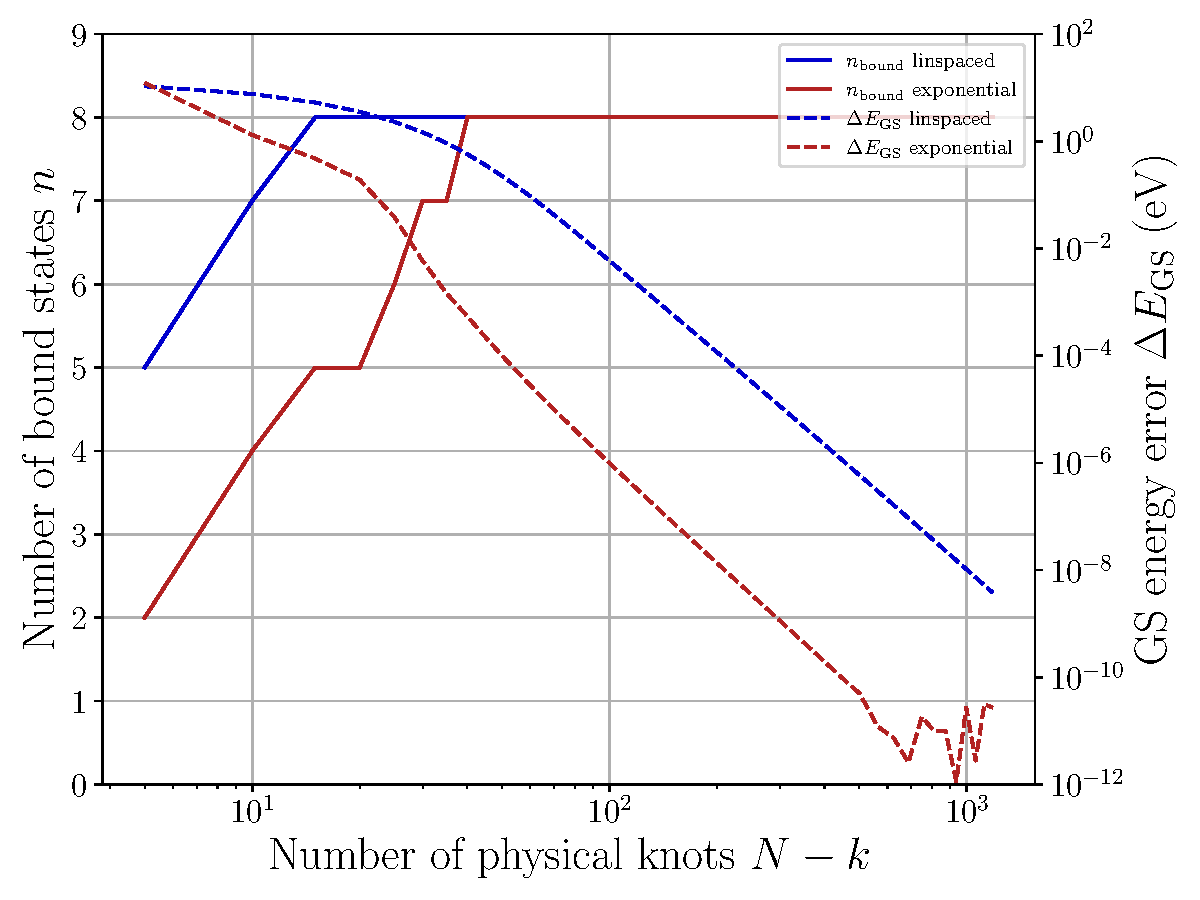
\includegraphics[width=0.65\textwidth]{../plots/ns_errs.pdf}
    \caption{Number of bound states found in the $l=0$ sector and the error of the ground state energy for linearly and exponentially spaced physical knots and varying number of knots. Exponentially spaced knots give a much lower error but also result in fewer states found for few knots.}
    \label{fig:nserrs}
\end{figure}
To combine the advantages of both approaches, we finally use points with an exponentially growing spacing
\begin{equation}
    r_{i+1} = r_i + \Delta r \cdot 10^{p_0 + i\cdot \Delta p}, \quad i = 1,\dots,N-k-1
\end{equation}
where with $\Delta r = 10^{-5}\,a_0$ and $N-k=1200$ physical points we obtain an $r_\text{max}$ of slightly larger than $100\,a_0$.

The maximum radius strongly impacts those states whose wave functions are highly extended compared to the maximally localised ground state. Especially as $l$ is increased, the states become increasingly long-reaching. This can be seen in figure~\ref{fig:ergerr} where the relative error of the numerically obtained energies is shown for all the bound states found with $l\leq 10$. States with small $n$ are more localised and the energy has a very small error, while for higher $n$ the error grows exponentially.

\begin{figure}
    \centering
    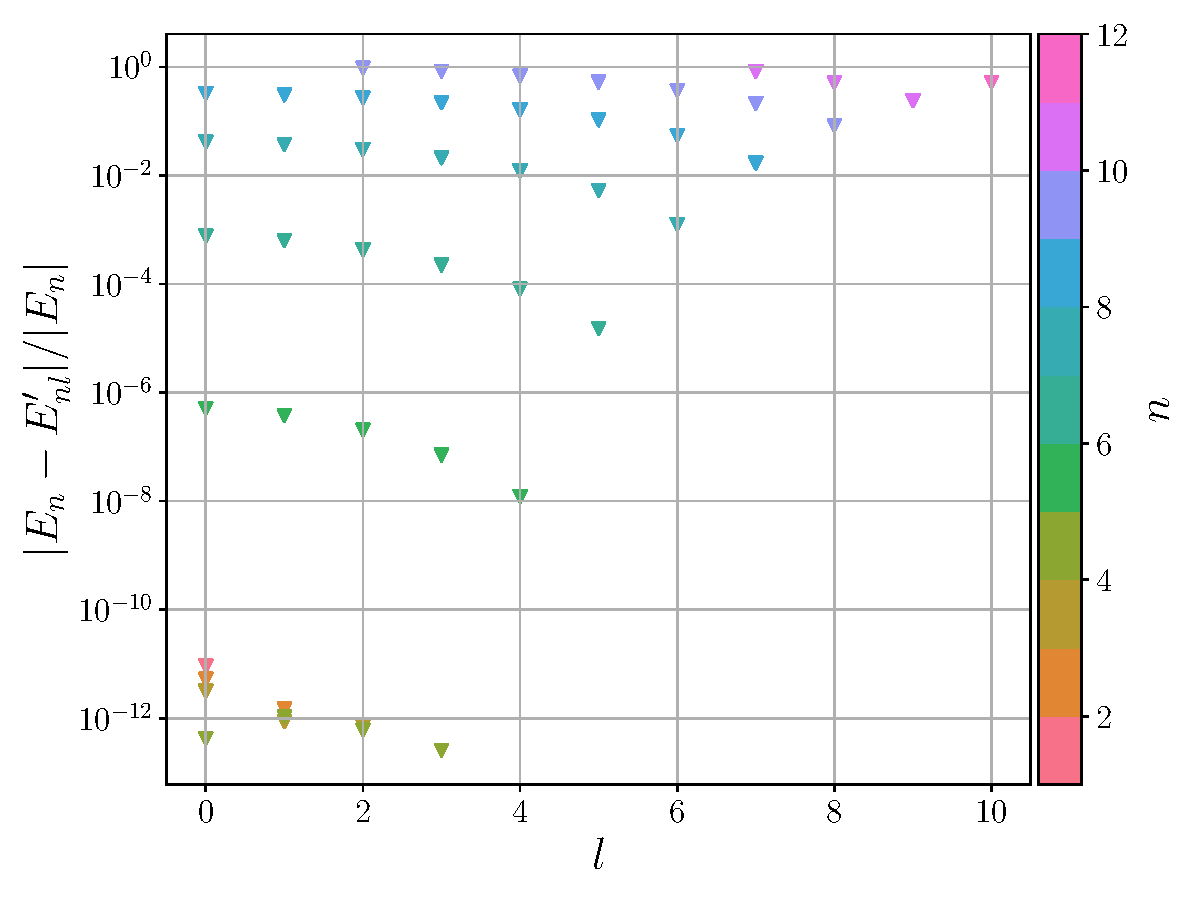
\includegraphics[width=0.65\textwidth]{../plots/erg_err.pdf}
    \caption{Relative error of the numerically obtained energies of all bound states found.}
    \label{fig:ergerr}
\end{figure}

\FloatBarrier
\section{Results}
Figure~\ref{fig:psi} shows the radial parts of the numerically obtained and exact wave functions for a selection of angular momenta $l$. $l=0$ states show a non-zero density in the nucleus at $r=0$, while states with $l>0$ go to zero in the origin. For larger $l$ and $n$ states which are significantly non-zero $[0, r_\text{max}]$ begin appearing. These are not well represented within the constraints of the algorithm and thus the states obtained deviate increasingly strongly from the exact solutions.

The solutions obey the knot theorem as expected.
\begin{figure}
    \centering
    \begin{subfigure}{0.49\textwidth}
        \centering
        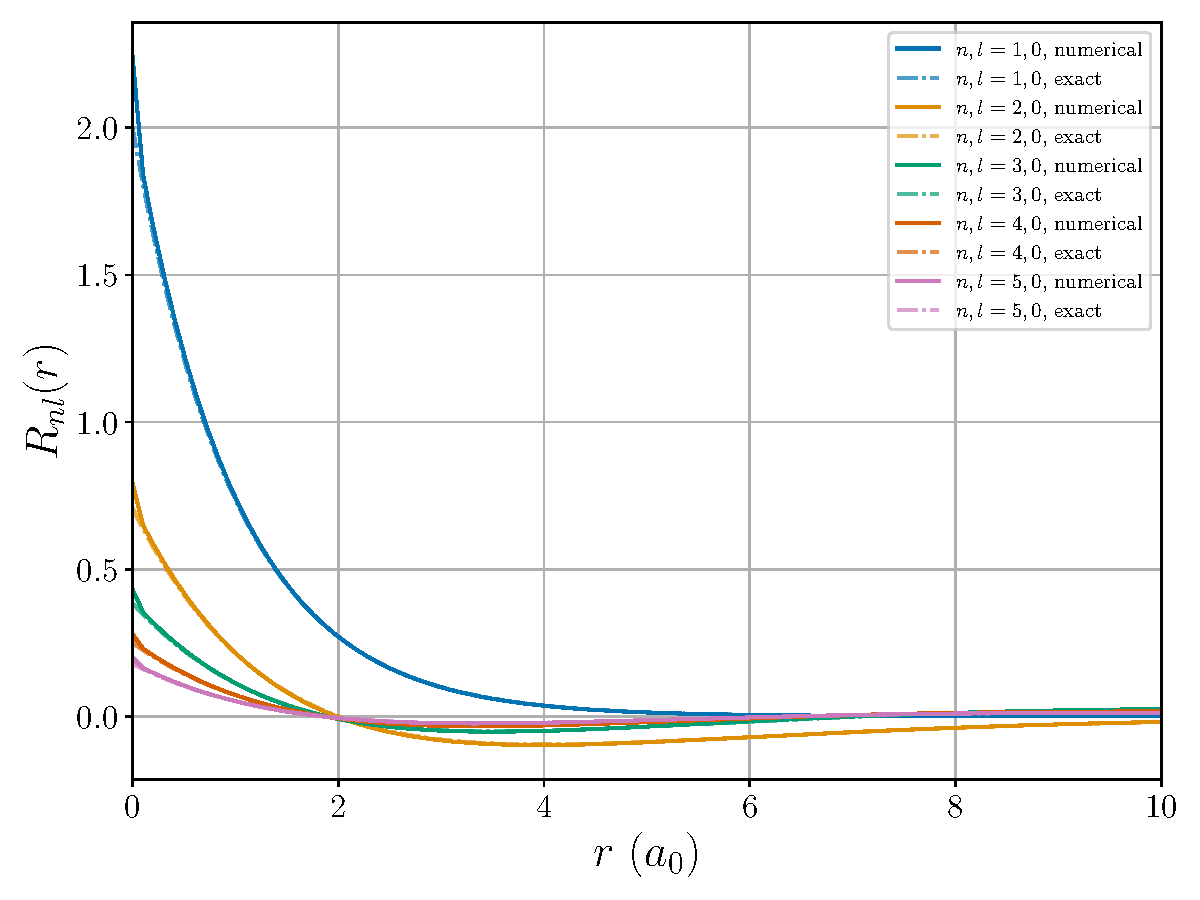
\includegraphics[width=\textwidth]{../plots/psis_comp/l0.pdf}
        \caption{$l=0$}
        \label{subfig:l0}
    \end{subfigure}
    \begin{subfigure}{0.49\textwidth}
        \centering
        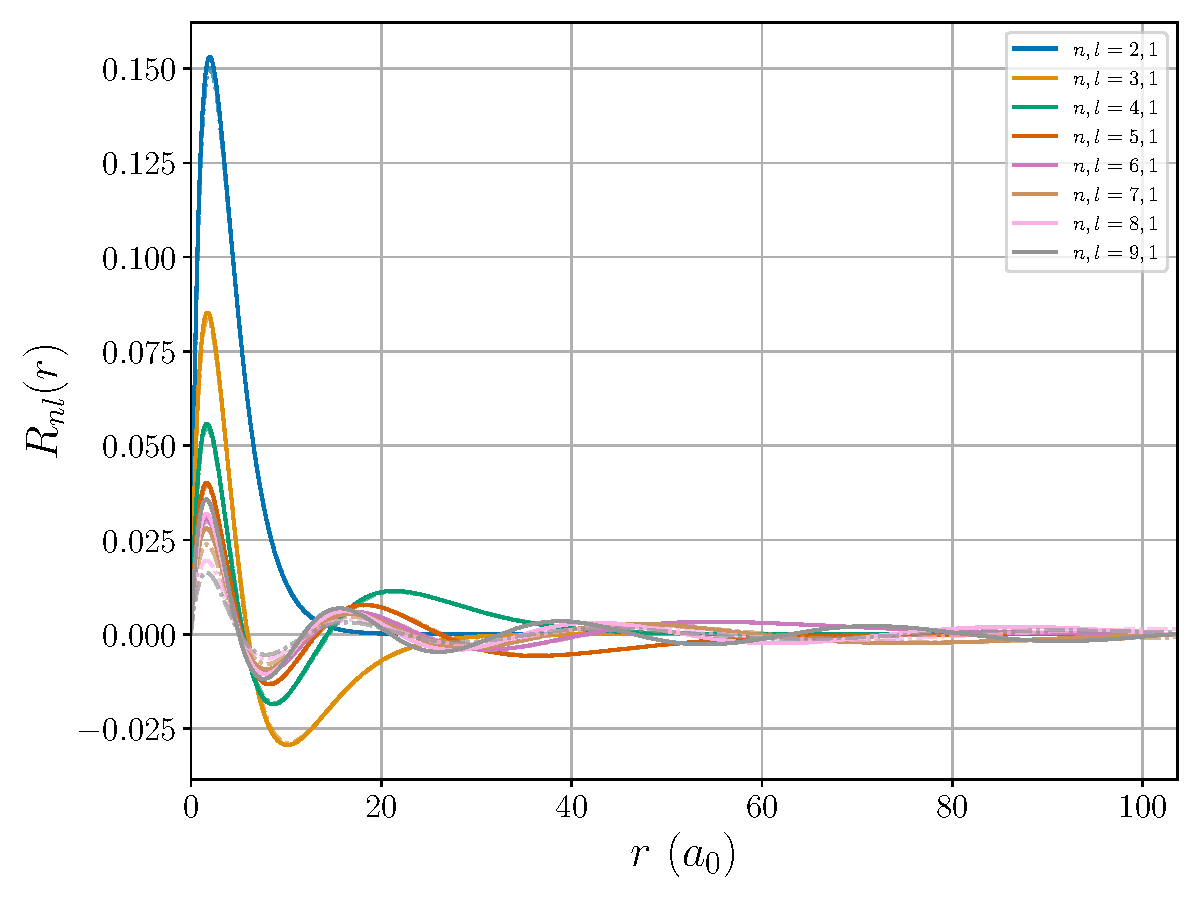
\includegraphics[width=\textwidth]{../plots/psis_comp/l1.pdf}
        \caption{$l=1$}
        \label{subfig:l1}
    \end{subfigure}
    \begin{subfigure}{0.49\textwidth}
        \centering
        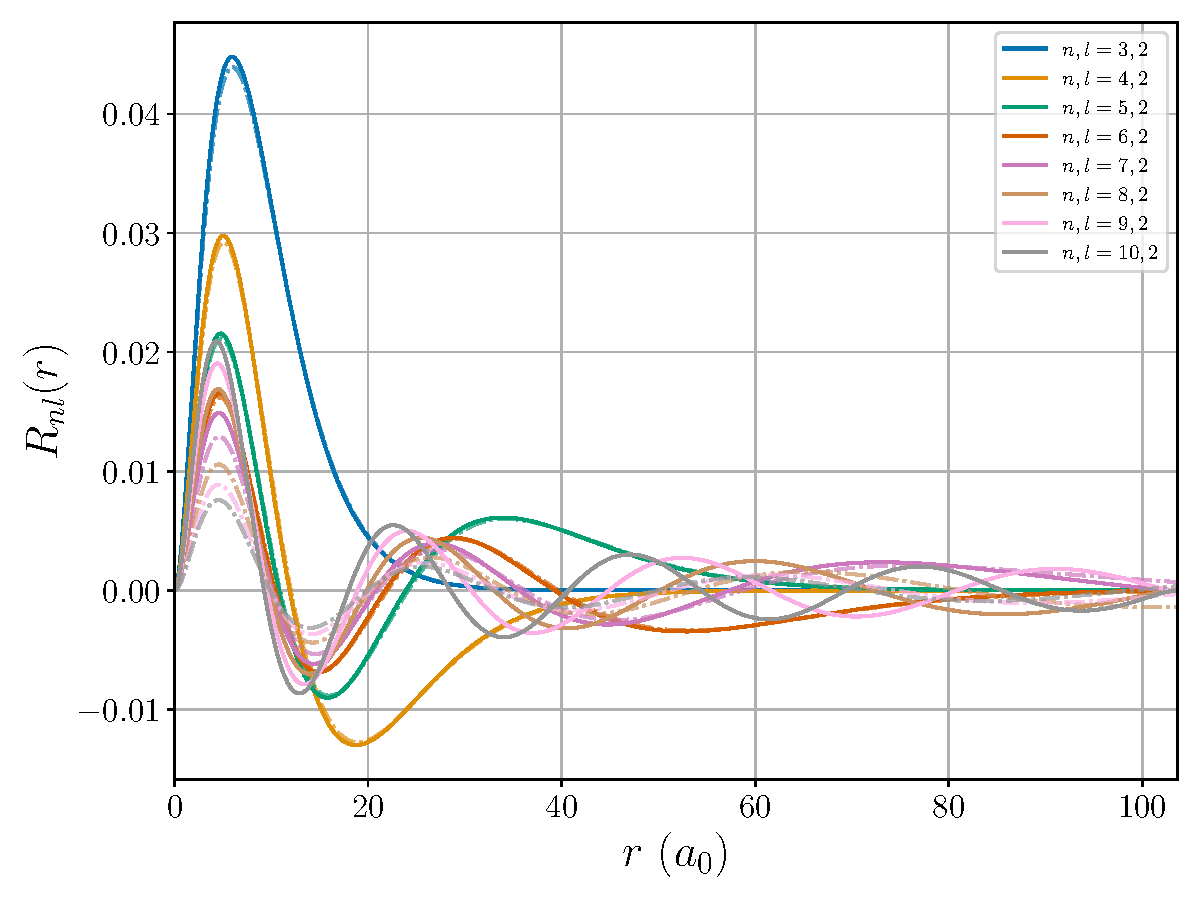
\includegraphics[width=\textwidth]{../plots/psis_comp/l2.pdf}
        \caption{$l=2$}
        \label{subfig:l2}
    \end{subfigure}
    \begin{subfigure}{0.49\textwidth}
        \centering
        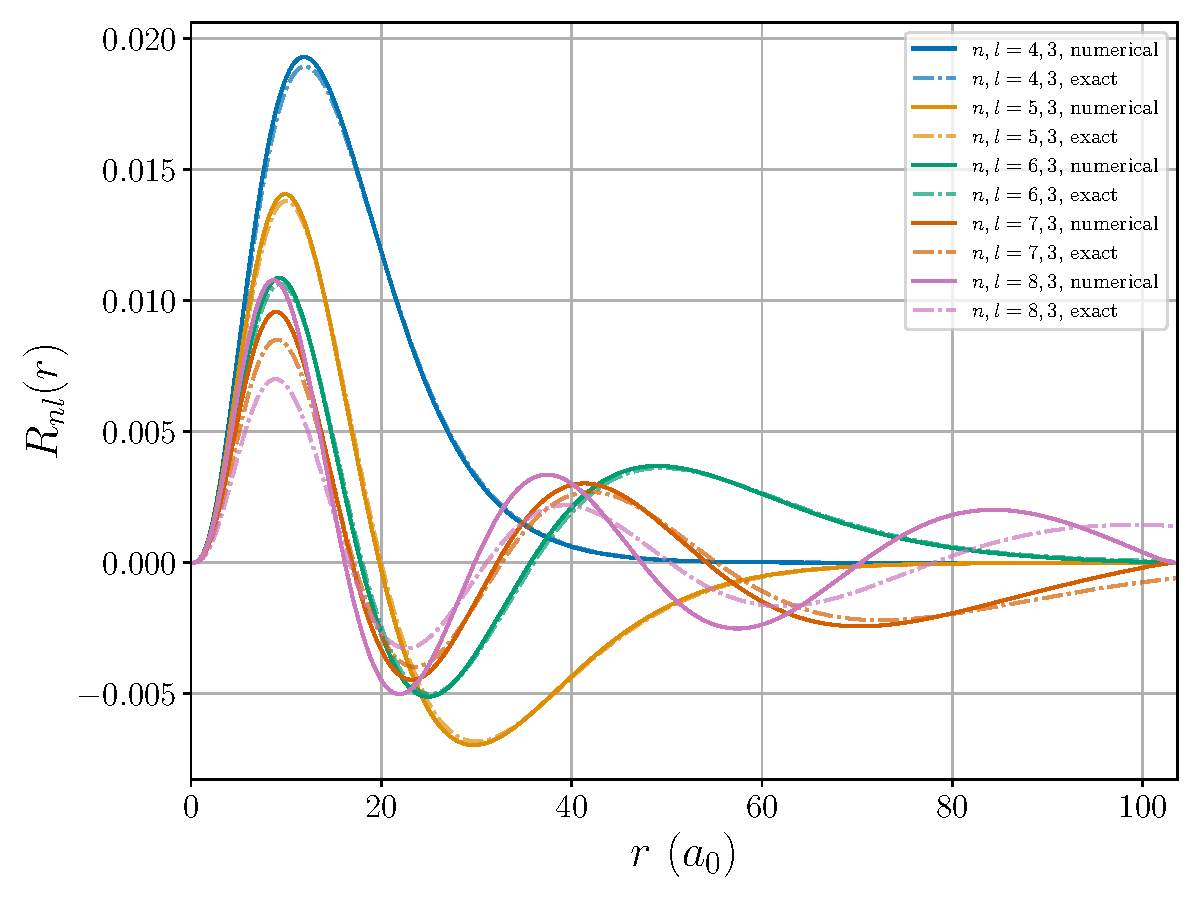
\includegraphics[width=\textwidth]{../plots/psis_comp/l3.pdf}
        \caption{$l=3$}
        \label{subfig:l3}
    \end{subfigure}\\
    \begin{subfigure}{0.49\textwidth}
        \centering
        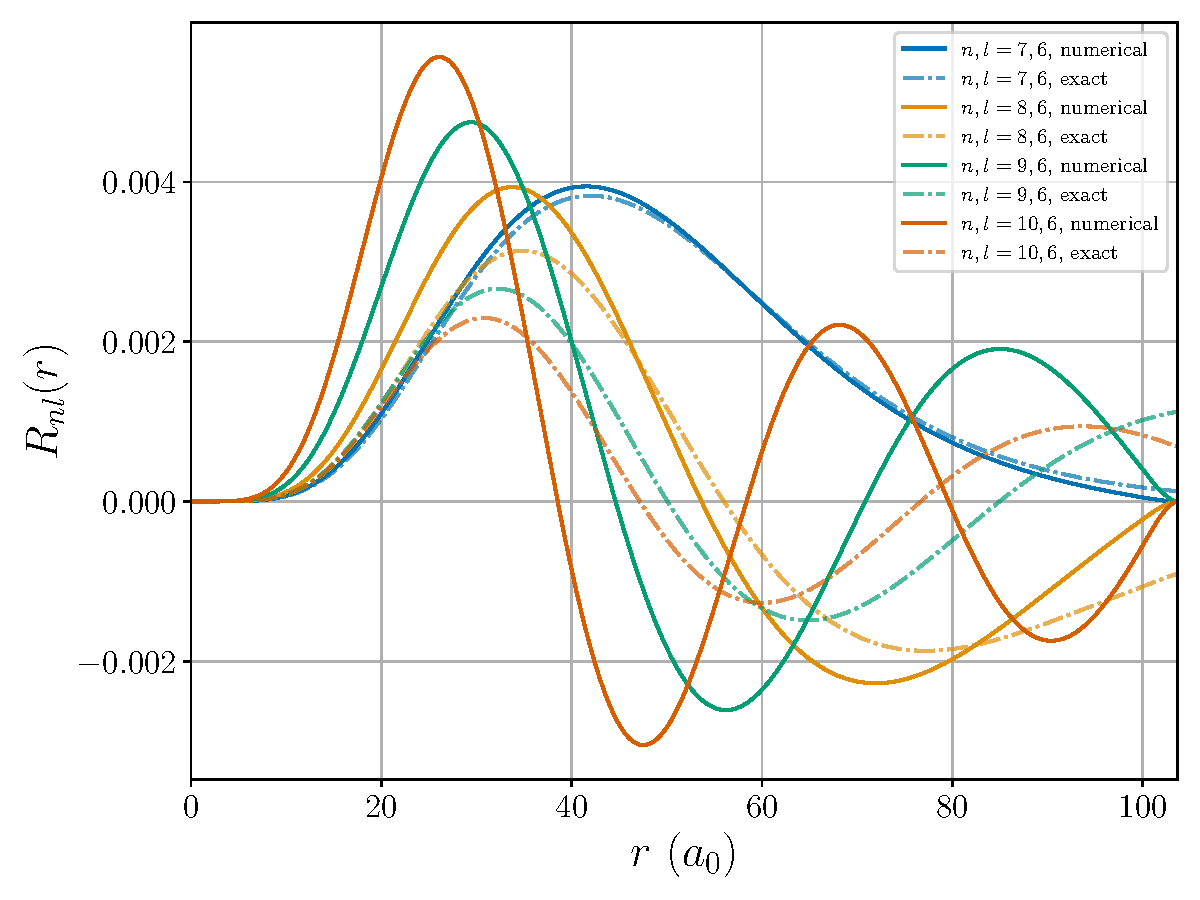
\includegraphics[width=\textwidth]{../plots/psis_comp/l6.pdf}
        \caption{$l=6$}
        \label{subfig:6}
    \end{subfigure}
    \begin{subfigure}{0.49\textwidth}
        \centering
        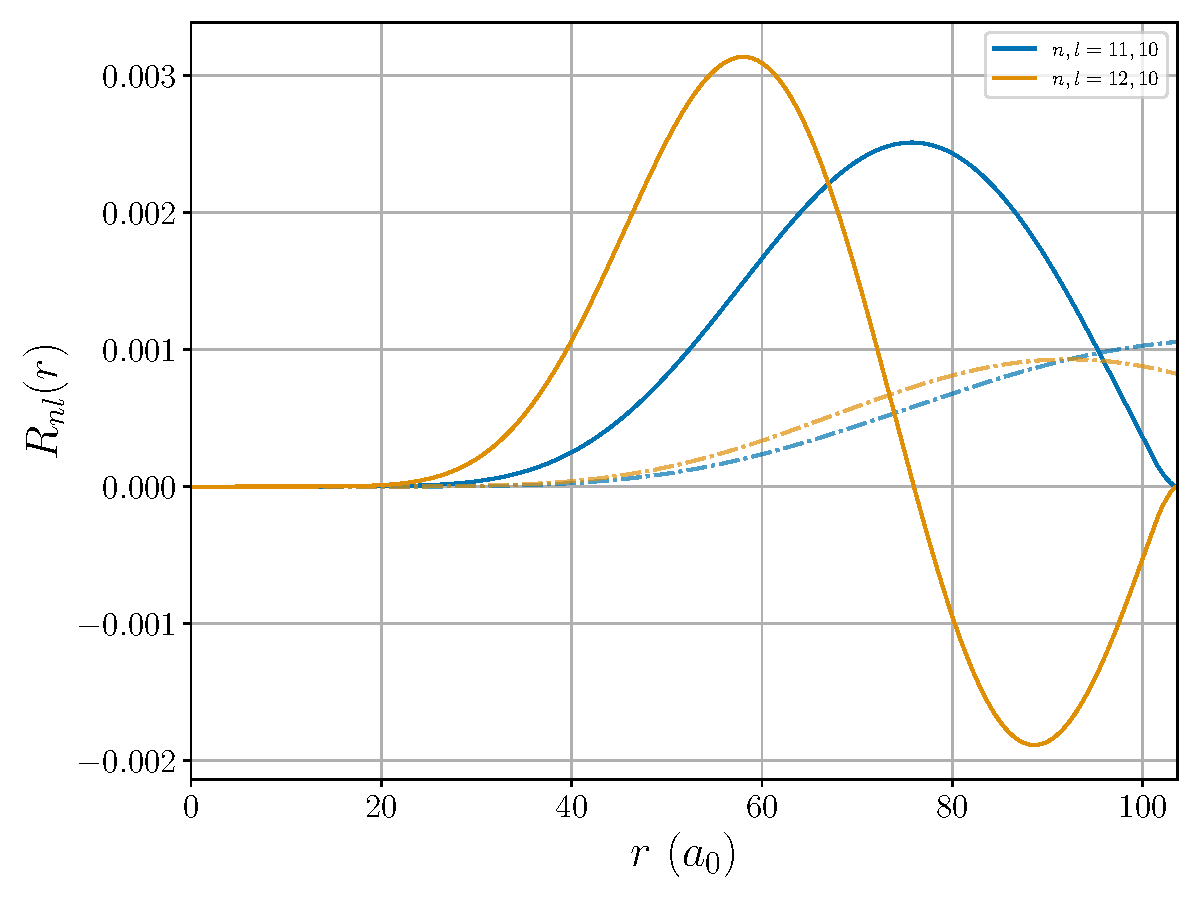
\includegraphics[width=\textwidth]{../plots/psis_comp/l10.pdf}
        \caption{$l=10$}
        \label{subfig:l10}
    \end{subfigure}
    \caption{First five numerical and exact wave functions for different $l$. $l=0$ states show a non-zero density in the nucleus at $r=0$, while states with $l>0$ go to zero in the origin. For larger $l$ states which do not \enquote{fit} into $[0, r_\text{max}]$ begin appearing. Note that these are also present in the smaller $l$ sectors but appear \enquote{later} and are thus not shown here.}
    \label{fig:psi}
\end{figure}

Figure~\ref{fig:erg} shows the energy spectrum of the states found up to $l=10$ in comparison to the exact energy eigenvalues. For smaller $l$ and $n$, the results agree well while for larger $n$ and $l$, the deviation increases.

\begin{figure}
    \centering
    \begin{subfigure}{0.49\textwidth}
        \centering
        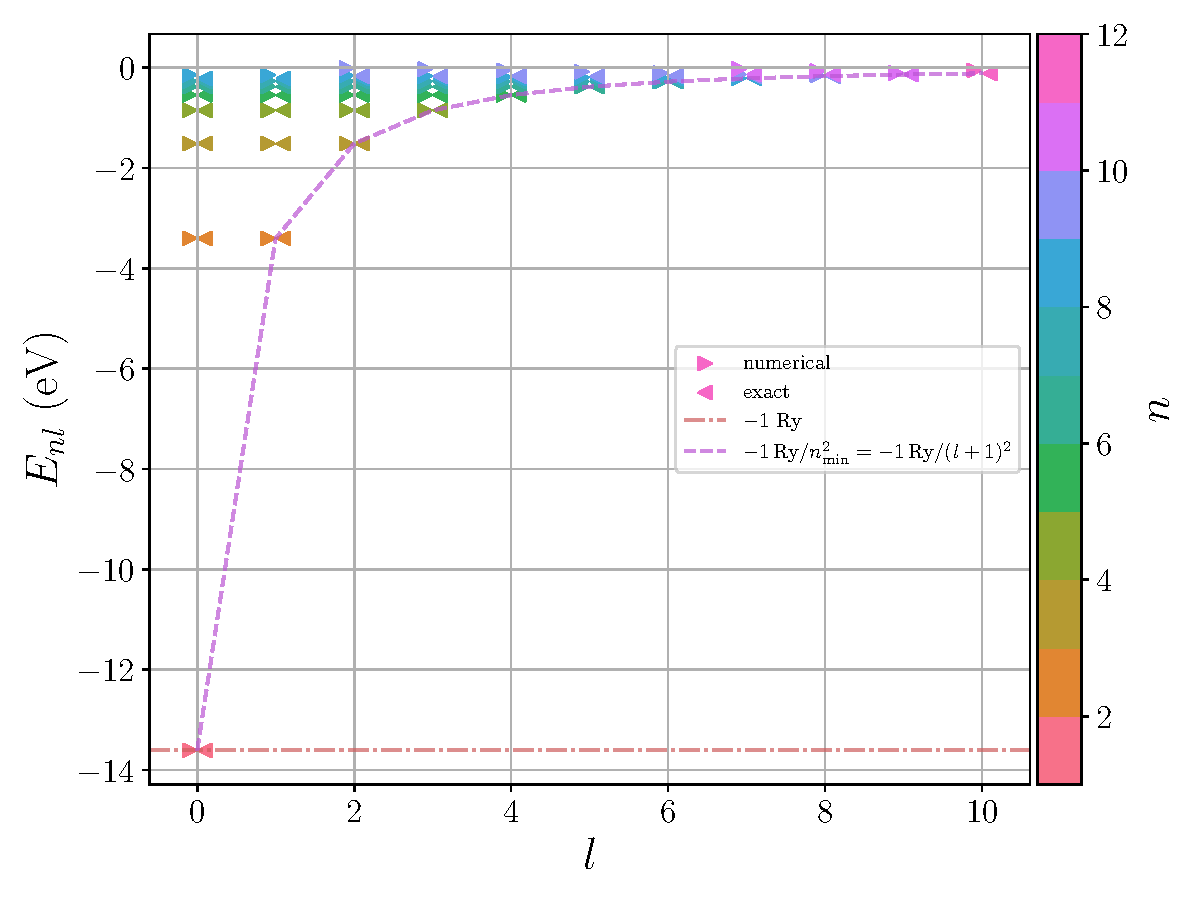
\includegraphics[width=\textwidth]{../plots/erg.pdf}
        \caption{Linear scale}
        \label{subfig:erg}
    \end{subfigure}
    \begin{subfigure}{0.49\textwidth}
        \centering
        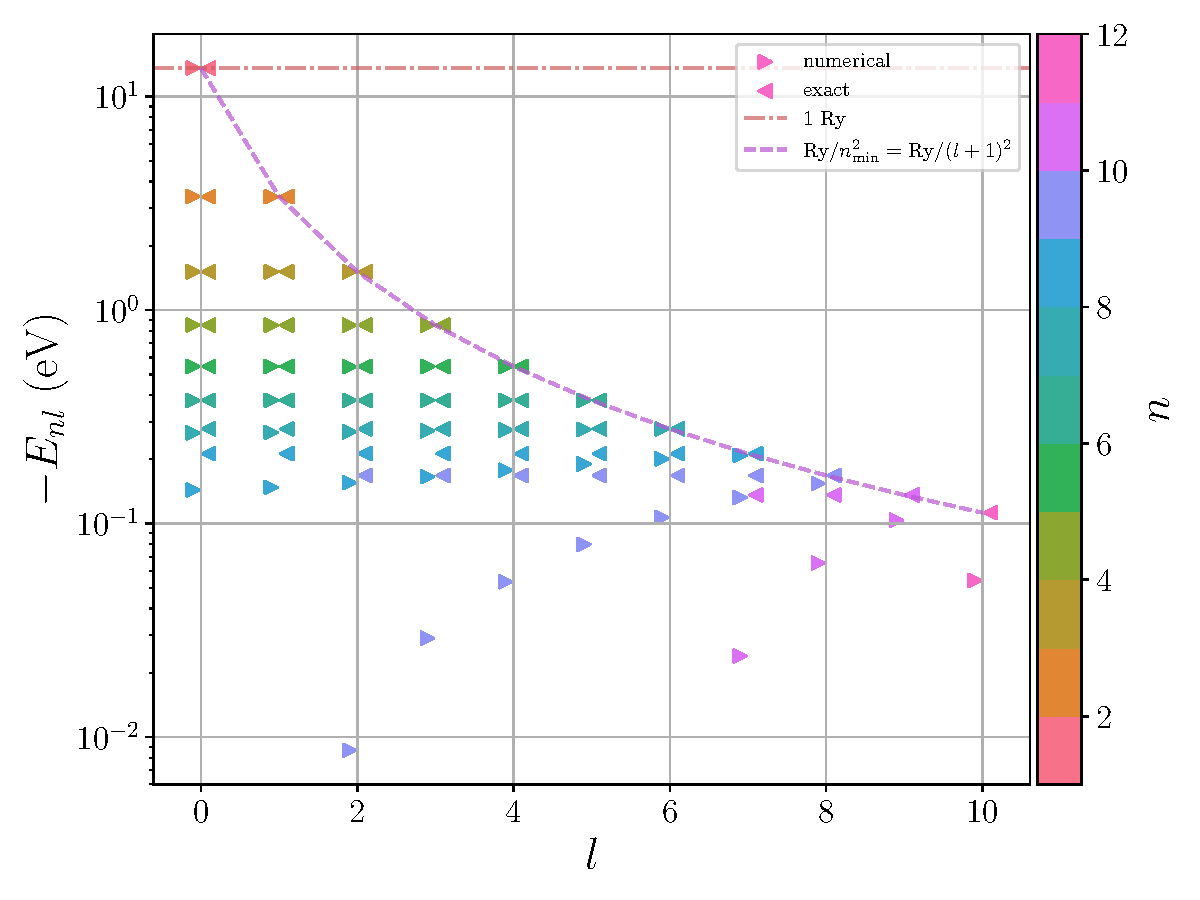
\includegraphics[width=\textwidth]{../plots/erg_log.pdf}
        \caption{Logarithmic scale}
        \label{subfig:erglog}
    \end{subfigure}
    \caption{Numerically obtained hydrogen energy spectrum, shown on a linear and a logarithmic scale for visual clarity. Comparison with the exact energies on the logarithmic scale shows that higher deviations begin to occur for larger $n$ and $l$ as expected.}
    \label{fig:erg}
\end{figure}
\FloatBarrier

\newpage
\section{Conclusion}
We are able to accurately compute the ground state of hydrogen and a good number of excited states, though higher lying states are increasingly less well represented on the finite interval if splines used. This could be remedied by adding more knot points at the expense of increased runtime. However, as was shown, there are diminishing returns when it comes to the amount of bound states found when adding more points.

If there had been more time, it would have been interesting to observe the effects of modifying the potential to include the effects of an extended core or to add relativistic corrections to $\mathcal{H}$.

\newpage
\fakesection{References}
\printbibliography


\end{document}
